\documentclass{article}
\usepackage{amsmath}
\usepackage{graphicx}
\usepackage[a4paper, margin=1in]{geometry}
\usepackage{pgfplots}
\pgfplotsset{compat=1.17}
\usepackage{afterpage}
\usepackage{float}
\usepackage{hyperref}
\usepackage{subcaption}
\graphicspath{{assets/}}

\title{Sorting arrays in parallel with Bitonic Sort using MPI}
\author{Eleni Koumparidou and Epameinondas Bakoulas}
\date{January 2025}

\begin{document}

\maketitle

\section{Objective}
Sorting algorithms usually take $O(nlogn)$ time to sort an array of size n. Bitonic sort is a parallel sorting 
algorithm that can sort very large arrays faster with the power of MPI and parallel processing. In this report, 
we will present the implementation of this algorithm. We will also present the results of our experiments 
and compare the different benchmarks.

\section{Algorithm Analysis}

\subsection{Overview}

Our goal is to sort an array of size $p * 2^q$, where $p = 2^k$, $k = [1:7]$ is the number of processes 
and $2^q$, $q = [20:27]$ the number of elements in each process.

\subsection{Parallelism - MPI}

The algorithm will follow the standard \textbf{Bitonic Sort Network} pattern as shown in Figure \ref{fig:bitonic-sort-network}.
Our goal is to create bitonic sequences of size $2, 4, 8, ..., p$ and then, with the correct exchanges between
processes, make bigger bitonic sequences. So our first step is to create bitonic sequences using 2 processes each time.
In order to do that, we will locally sort the processes in ascending/descending order using \texttt{quickSort (qsort)}.
This step is quite costly but it is necessary for the algorithm and we will only do it once.

Now we can start the communications between the processes. Each process will keep either the \texttt{min} or
\texttt{max} elements element wise. Once this finishes, every process (block) will be a bitonic sequence, so we can sort 
them locally in O(n) time by applying the \texttt{elbowSort} algorithm explained in detail later on.

We repeat this process but now we initally communicate with the neighbors of distance 2, and then with 
the neighbors of distance 1. The sorting always takes place right after we communicate with the closest neighbor.
In total, this process is repeated $\log_2{p}$ times, and each time we double the initial distance. 
This is clearly visible in Figure \ref{fig:bitonic-sort-network}, where the total steps are equal to $\log_2{8} = 3$.

Finally, we end up with $p$ processes sorted in ascending order, and if we merge them together we get a fully
sorted array of size $p * 2^q$.

\begin{figure}[H]
\begin{verbatim}
void bitonicSort(int rank, int num_p, int num_q, int **array) {
    // Initial sorting of the processes
    sortProcesses(rank, num_q, *array);
    for (int group_size = 2; group_size <= num_p; group_size *= 2) {
        bool sort_descending = rank & group_size;
        for (int distance = group_size / 2; distance > 0; distance /= 2) {
            int partner_rank = rank ^ distance;
            minmax(rank, partner_rank, num_q, *array, sort_descending);
        }
        elbowMerge(num_p, num_q, array, sort_descending);
    }
}
\end{verbatim}
\caption{Bitonic Sort Algorithm. The function sortProcesses sorts each process using quick sort, while the
minmax function exchanges the min/max elements between two processes. Finally, the elbowMerge function sorts
the bitonic sequence locally.}
\label{alg:bitonic-sort}
\end{figure}


\begin{figure}[H]
    \centering
    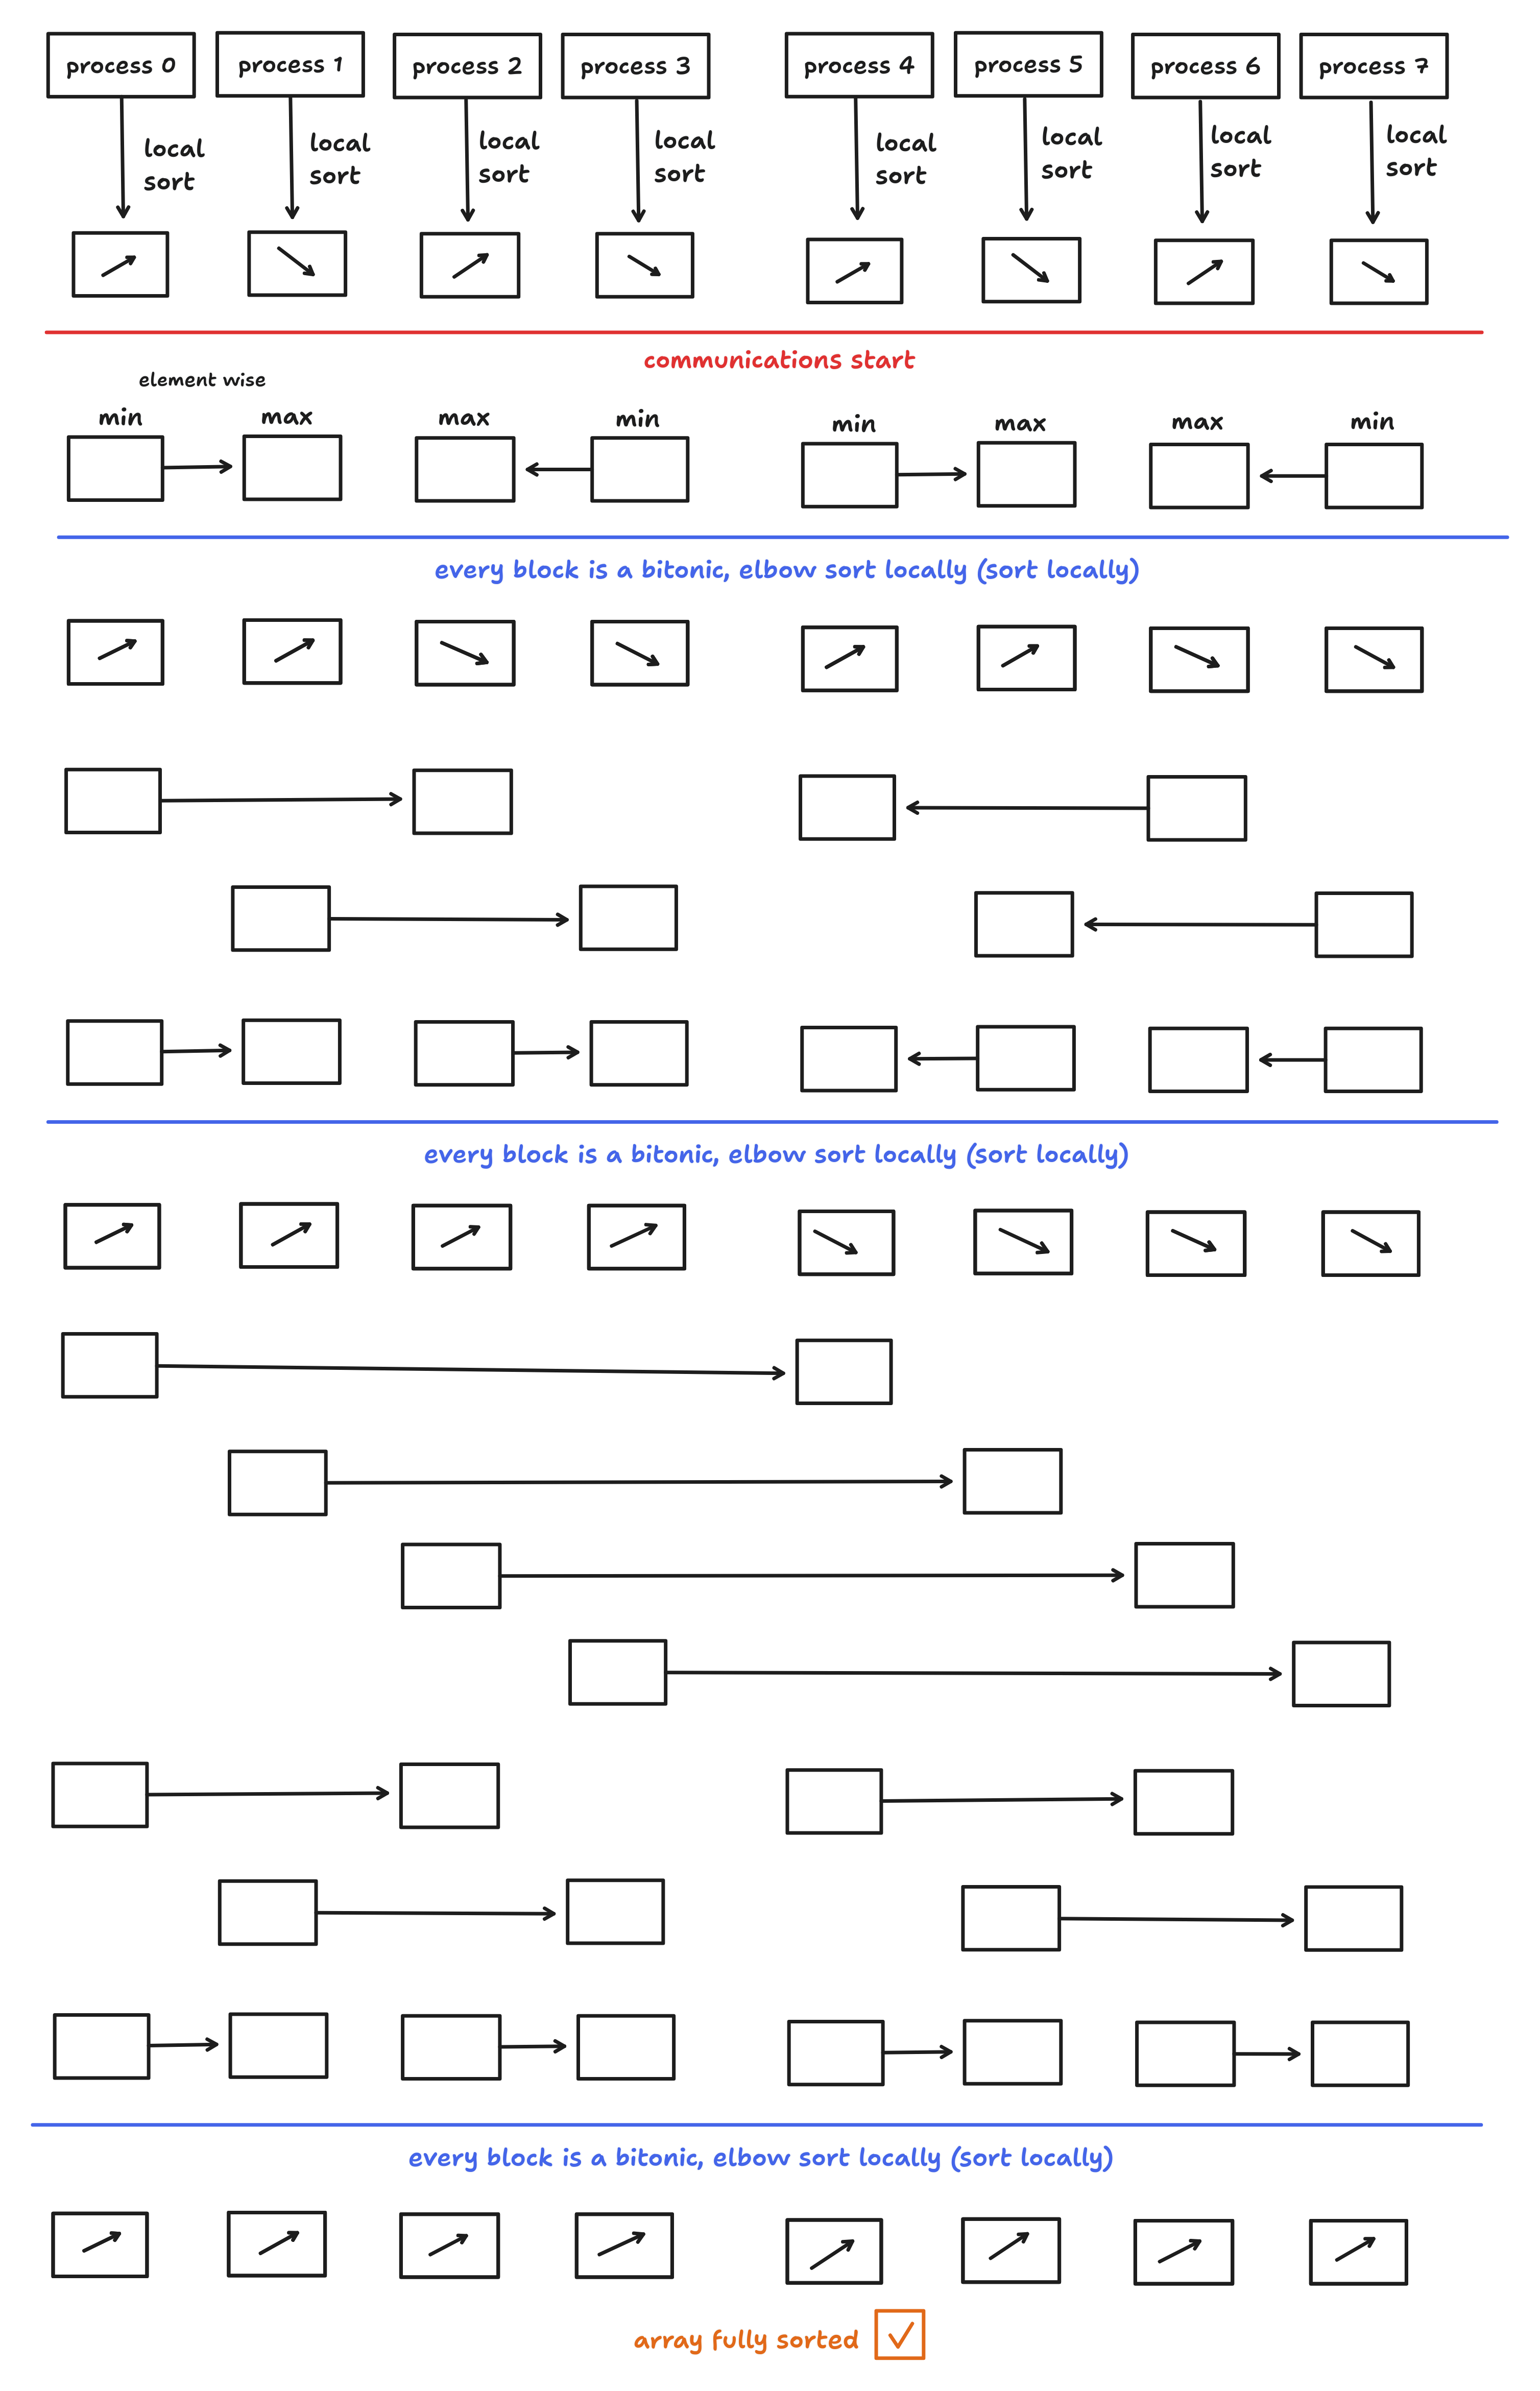
\includegraphics[width=0.9\textwidth]{bitonic-sort-network.png}
    \caption{Bitonic Sort Network}
    \label{fig:bitonic-sort-network}
\end{figure}


\subsection{Hypercube model}

Finding the right neighbor to exchange data with in each stage of the algorithm can be quite tricky. One possible way
is to leverage the power of the hypercube model. First, we give each process a unique $log_2{p}$ bit id. In the case
of 8 processes, each process will have a 3 bit id, as shown in Figure \ref{fig:hypercube-model}. In order to find the right neighbor, all we
need to do is compute $$pid \oplus distance$$ where $\oplus$ is the XOR (exclusive-OR) operator and $pid$ the process id.

\begin{figure}[h]
    \centering
    
    \begin{subfigure}[b]{0.45\textwidth}
        \centering
        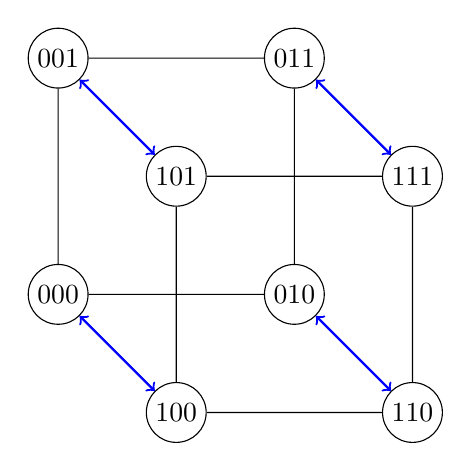
\begin{tikzpicture}[scale=1.5, every node/.style={circle, draw, fill=white, inner sep=2pt, text centered}]
            % 1st Cube (Upper Left)
            \node (3D-1) at (1,-3.5) {000};
            \node (3D-2) at (1,-1.5) {001};
            \node (3D-3) at (3,-3.5) {010};
            \node (3D-4) at (3,-1.5) {011};
            \node (3D-5) at (2,-4.5) {100};
            \node (3D-6) at (2,-2.5) {101};
            \node (3D-7) at (4,-4.5) {110};
            \node (3D-8) at (4,-2.5) {111};
            
            % Edges for the first cube (Upper Left)
            \draw (3D-1) -- (3D-2);
            \draw (3D-2) -- (3D-4);
            \draw (3D-4) -- (3D-3);
            \draw (3D-3) -- (3D-1);
            \draw [<->, thick, draw=blue] (3D-1) -- (3D-5);
            \draw [<->, thick, draw=blue] (3D-2) -- (3D-6);
            \draw [<->, thick, draw=blue] (3D-3) -- (3D-7);
            \draw [<->, thick, draw=blue] (3D-4) -- (3D-8);
            \draw (3D-5) -- (3D-6);
            \draw (3D-6) -- (3D-8);
            \draw (3D-8) -- (3D-7);
            \draw (3D-7) -- (3D-5);
        \end{tikzpicture}
        \caption{Communications at distance 4}
    \end{subfigure}
    \hfill
    \begin{subfigure}[b]{0.45\textwidth}
        \centering
        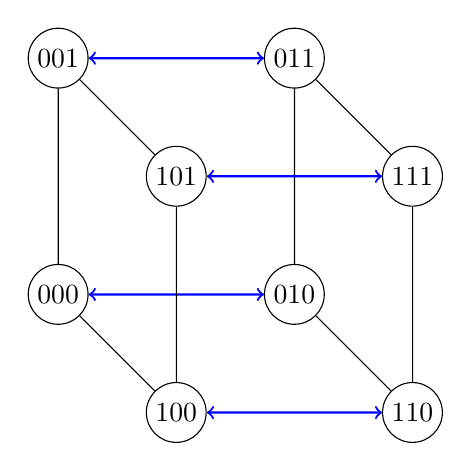
\begin{tikzpicture}[scale=1.5, every node/.style={circle, draw, fill=white, inner sep=2pt, text centered}]
            % 2nd Cube (Upper Right)
            \node (3D-9) at (6,-3.5) {000};
            \node (3D-10) at (6,-1.5) {001};
            \node (3D-11) at (8,-3.5) {010};
            \node (3D-12) at (8,-1.5) {011};
            \node (3D-13) at (7,-4.5) {100};
            \node (3D-14) at (7,-2.5) {101};
            \node (3D-15) at (9,-4.5) {110};
            \node (3D-16) at (9,-2.5) {111};
            
            % Edges for the second cube (Upper Right)
            \draw (3D-9) -- (3D-10);
            \draw[<->, thick, draw=blue] (3D-10) -- (3D-12);
            \draw (3D-12) -- (3D-11);
            \draw[<->, thick, draw=blue] (3D-11) -- (3D-9);
            \draw (3D-9) -- (3D-13);
            \draw (3D-10) -- (3D-14);
            \draw (3D-11) -- (3D-15);
            \draw (3D-12) -- (3D-16);
            \draw (3D-13) -- (3D-14);
            \draw[<->, thick, draw=blue] (3D-14) -- (3D-16);
            \draw (3D-16) -- (3D-15);
            \draw[<->, thick, draw=blue] (3D-15) -- (3D-13);
        \end{tikzpicture}
        \caption{Communications at distance 2}
    \end{subfigure}
    \hfill
    \begin{subfigure}[b]{0.6\textwidth}
        \centering
        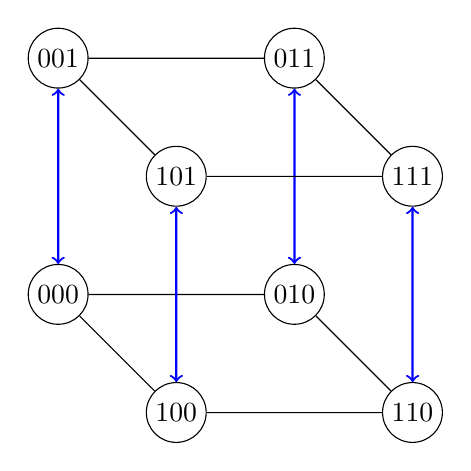
\begin{tikzpicture}[scale=1.5, every node/.style={circle, draw, fill=white, inner sep=2pt, text centered}]
            % 3rd Cube (Lower Middle)
            \node (3D-17) at (4,-7.5) {000};
            \node (3D-18) at (4,-5.5) {001};
            \node (3D-19) at (6,-7.5) {010};
            \node (3D-20) at (6,-5.5) {011};
            \node (3D-21) at (5,-8.5) {100};
            \node (3D-22) at (5,-6.5) {101};
            \node (3D-23) at (7,-8.5) {110};
            \node (3D-24) at (7,-6.5) {111};
            
            % Edges for the third cube (Lower Middle)
            \draw[<->, thick, draw=blue] (3D-17) -- (3D-18);
            \draw (3D-18) -- (3D-20);
            \draw[<->, thick, draw=blue] (3D-20) -- (3D-19);
            \draw (3D-19) -- (3D-17);
            \draw (3D-17) -- (3D-21);
            \draw (3D-18) -- (3D-22);
            \draw (3D-19) -- (3D-23);
            \draw (3D-20) -- (3D-24);
            \draw[<->, thick, draw=blue] (3D-21) -- (3D-22);
            \draw (3D-22) -- (3D-24);
            \draw[<->, thick, draw=blue] (3D-24) -- (3D-23);
            \draw (3D-23) -- (3D-21);
        \end{tikzpicture}
        \caption{Communications at distance 1}
    \end{subfigure}
    
    \caption{(Hyper)cube model with 8 processes.}
    \label{fig:hypercube-model}
\end{figure}

\subsection{Elbow sort}
\texttt{ElbowSort} sorts efficiently a bitonic sequence in \textbf{O(n)} time:
\begin{itemize}
\item
The minimum element of the bitonic sequence, known as the \textbf{elbow}, is found in \textbf{linear time} and depending on the order of the sorting, it is placed as the first or last element of the sorted array.
\item 
The array is scanned in a circular way, by placing a \texttt{left} and a \texttt{right} pointer to the left and right of the elbow. This means that when one pointer reaches the end of the array, it loops around to the other end.  
\end{itemize}
During the scanning process, the smallest of the two elements pointed is placed in the sorted array and the corresponding pointer moves to the next element, until all elements have been placed into the sorted array in \textbf{linear time} again. The sorting direction (ascending or descending) and the placement of the elbow (first or last) are determined by the ID of the process combined with the phase of the procedure, as shown in Figure \ref{fig:bitonic-sort-network}.

\section{Benchmarks}
Different testings took place in \textbf{rome partition} of \href{https://hpc.it.auth.gr/}{\textbf{Aristotel Cluster}} to test the performance of our sorting algorithm, inlcluding efficiency and speed. To ensure that valid results were provided, we developed a function \texttt{evaluateResult}, which compares only the last element of a process and the first element of the next one to confirm that the global array is sorted.

\subsection{Performance}


\subsection{Parallel processing}
The performance of sorting 2\textsuperscript{27} elements across different processes is presented in Table \ref{tab:acceleration}. The speedup is calculated by comparing the execution time to that of a single process, which is equivalent to using quick sort. In the case of 128 processes, the execution time is almost \textbf{10 times reduced}. This confirms that increasing the number of processes accelerates the algorithm's execution.
\begin{table}[h!]
\centering
\begin{tabular}{|c|c|c|c|c|c|c|c|c|}
\hline
\textbf{processes} & 1 & 2 & 4 & 8 & 16 & 32 & 64 & 128 \\
\hline
\textbf{speedup} & 1 & 1.84 & 3.05 & 4.64 & 4.67 & 6.14& 7.70 & 9.56 \\
\hline
\textbf{time} & 14.105497 & 7.637068 & 4.612354 & 3.035330 & 3.014933 & 2.296470 & 1.830522 & 1.474246 \\
\hline
\end{tabular}
\caption{Performance for 2\textsuperscript{27} elements across different processes.}
\label{tab:acceleration}
\end{table}

\subsection{Using Nodes}
In Figure \ref{fig:proc vs nodes}, we analyzed the sorting of $q = [20:27]$ elements while increasing the number of nodes used for the partition. We observed a significant reduction in execution time, with a decrease of up to 50\% for 8 nodes.

\begin{figure}[h!]
    \centering
    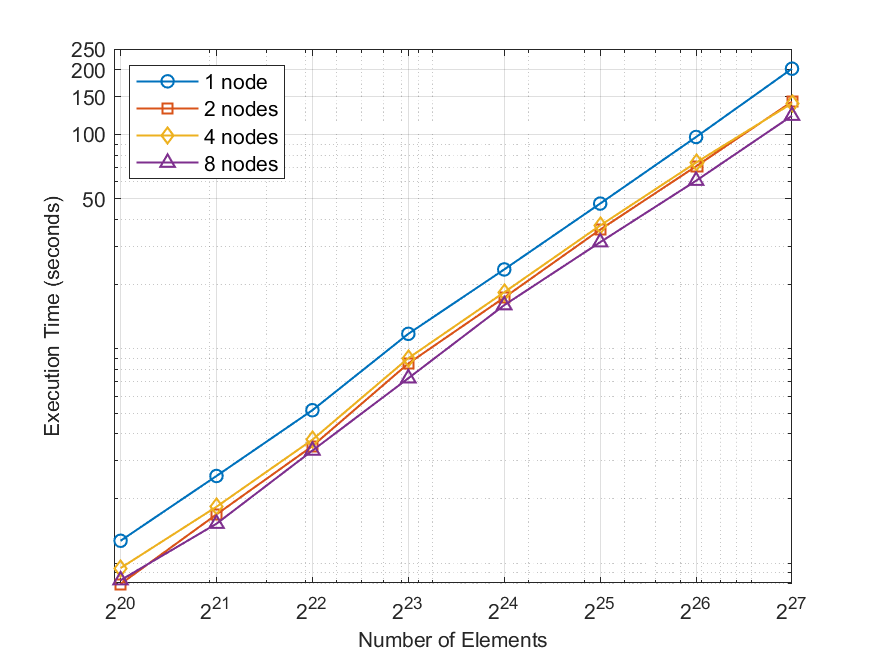
\includegraphics[width=1\linewidth]{execution_time_vs_elements.png}
    \caption{Execution time using different number of nodes}
    \label{fig:proc vs nodes}
\end{figure}



\end{document}
